\documentclass[../practica_06.tex]{subfiles}

\begin{document}

    \begin{enumerate}
        \item $f(x,y) = x^2 + y^2 -2x$
        
            \begin{itemize}
                \item $f_x(x,y) = 2x - 2 $
                \item $f_y(x,y) = 2y$
            \end{itemize}

            $\grad f(x,y) = (0,0) \Leftrightarrow$

            $\left\{
            \begin{array}{ll}
                2x -2 = 0\\
                2y = 0
            \end{array}
            \right. \Leftrightarrow (x,y) = (1,0)$

            $H_f(x,y) = \begin{vmatrix}
                2 & 0 \\
                0 & 2
            \end{vmatrix} \wedge det(H_f(x,y)) = 4$

            Por el criterio es un minimo local

            $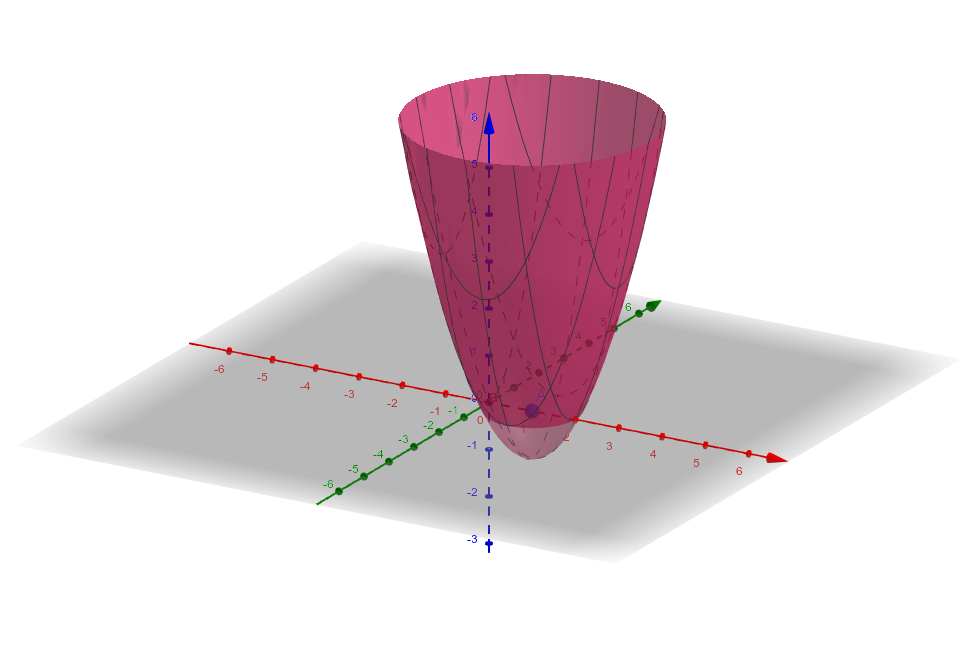
\includegraphics[scale=0.4]{ej05/resources/5a.png}$

        \item $f(x,y) = x^2 + y^2 + x^2y + 4 \wedge D=\{(x,y)\in \mathbb{R}^2: \abs*{x}\leq 1 \wedge \abs*{y}\leq 1\}$

            $D$ compactor y $f(x,y)$ continua $\Rightarrow$ f(x,y) alcanza su maximo y minimo en D por waiertrass

            $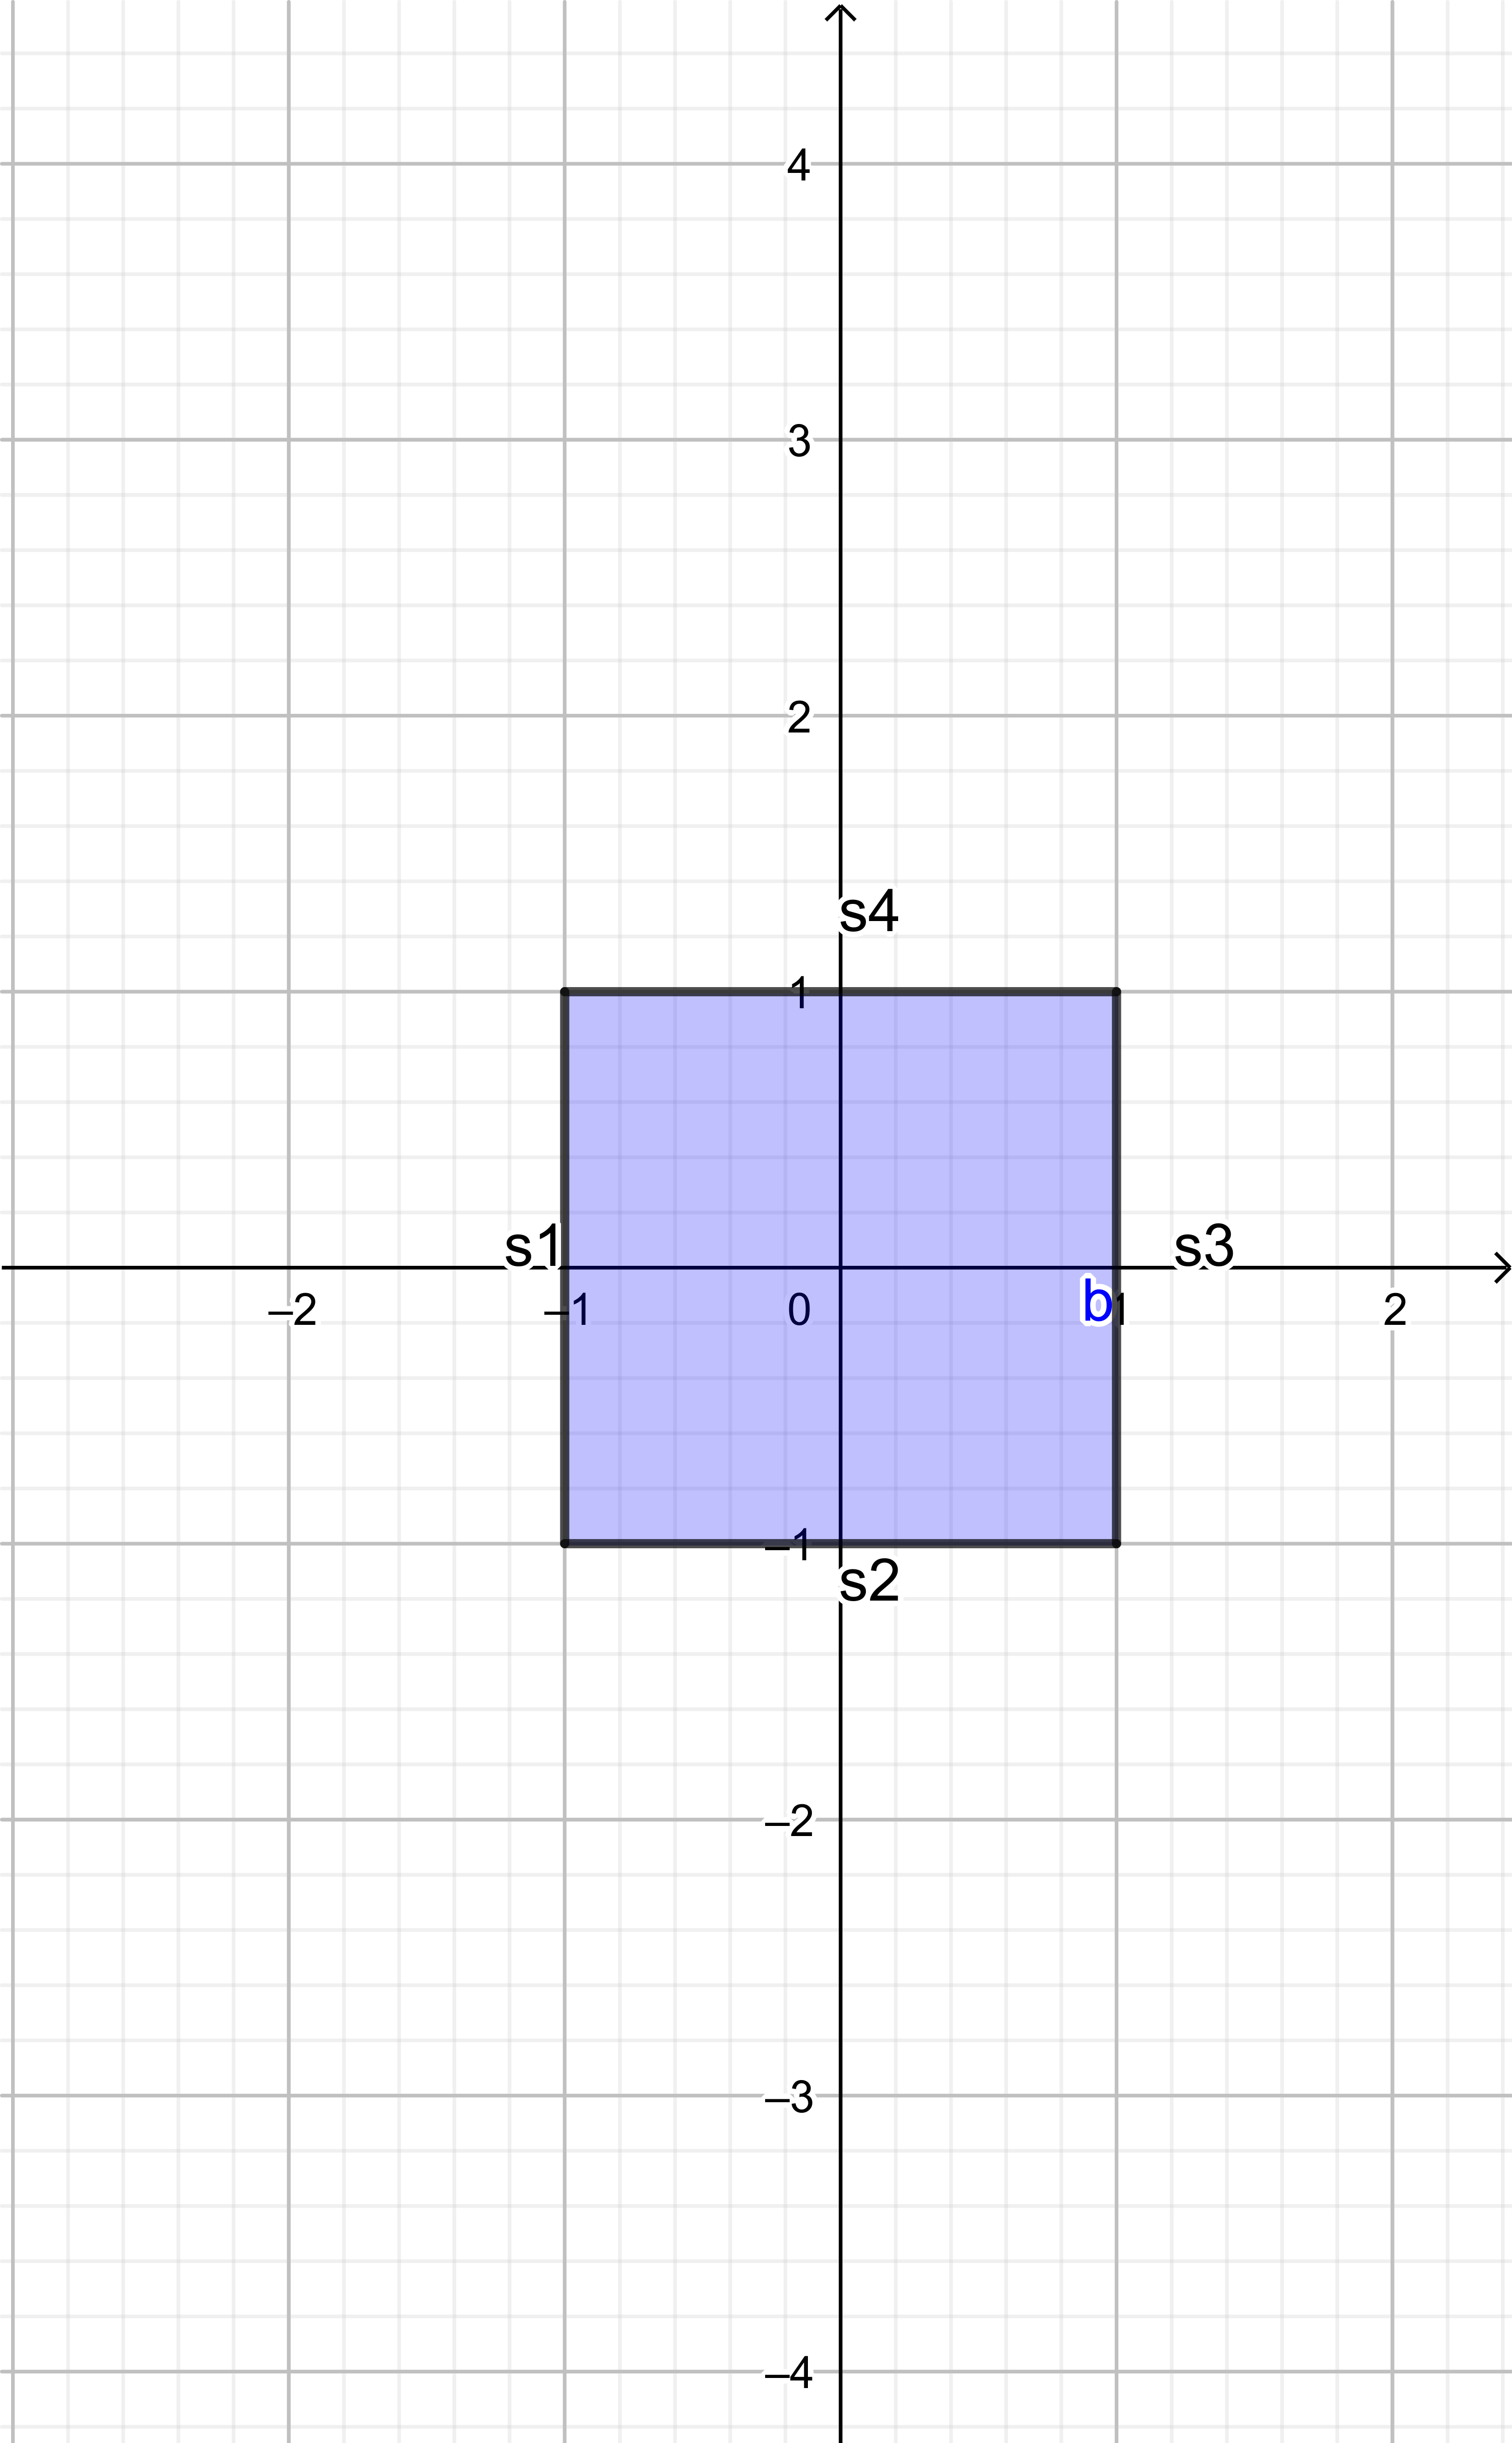
\includegraphics[scale=0.4]{ej05/resources/5bd.png}$

            \subsection*{Interior de $D$}

            \begin{itemize}
                \item $f_x(x,y) = 2x + 2xy$
                \item $f_y(x,y) = 2y + x^2$
            \end{itemize}

            $\grad f(x,y) = (0,0) \Leftrightarrow$

            $\left\{\begin{array}{ll}
                2x + 2xy = 0 \Rightarrow 2x + x^3 = 0 \Leftrightarrow x(2+x^2) = 0 \Leftrightarrow x = 0 \vee x = \pm \sqrt{2}\\
                2y + x^2 = 0 \Rightarrow y = \frac{x^2}{2}
            \end{array}
            \right. \Rightarrow$

            Ptos criticos = $ (0, 0), \stackrel{\notin D}{\cancel{(\sqrt{2},1), (-\sqrt{2},1)}}$

            \subsection*{Borde de $D$}

            \subsubsection*{S1}

            $f(-1,y) = y^2 + y + 5 = g(y) \wedge y \in [-1,1]$

            $g^{\prime}(y) = 2y + 1 = 0 \Leftrightarrow (x,y) = (-1,-\frac{1}{2})$

            \subsubsection*{S2}

            $f(x,-1) = \cancel{x^2} + 1 \cancel{- x^2} + 4 = 5 = h(x) \wedge x \in [-1,1]$

            $h^{\prime}(x) = 0 \Rightarrow (x,-1) \wedge x \in [-1,1] $

            \subsubsection{S3}

            $f(1,y) = 1 + y^2 + y + 4 = h(x)$

            \subsubsection*{S4}

            $f(x,1) = 2x^2 + 5 = i(x) \wedge x \in [-1,1]$

            $i^{\prime}(x) = 4x = 0 \Leftrightarrow (x,y) = (0,1)$


            \subsection*{Ptos criticos}

            \begin{itemize}
                \item $(0,0) \Rightarrow f(0,0) = 4$
                \item $(-1,-\frac{1}{2}) \Rightarrow f(-1,-\frac{1}{2}) = 1 + \frac{1}{4} + \frac{1}{2} + 4 = 5 + \frac{3}{4} $
                \item $(x,-1) \Rightarrow f(x,-1)= 5$
                \item $(0,1) \Rightarrow f(0,1) = 5$
                \item $(1,1) \Rightarrow f(1,1) = 7$
                \item $(-1,1) \Rightarrow f(-1,1) = 7$
                \item $(-1,-1) \Rightarrow f(-1,-1) = 5$
                \item $(1,-1) \Rightarrow f(-1,-1) = 5$
            \end{itemize}

            \begin{itemize}
                \item $\max f = 7$ en los puntos $(1,1)\wedge(-1,1)$
                \item $\max f = 4$ en el punto $(0,0)$
            \end{itemize}

            $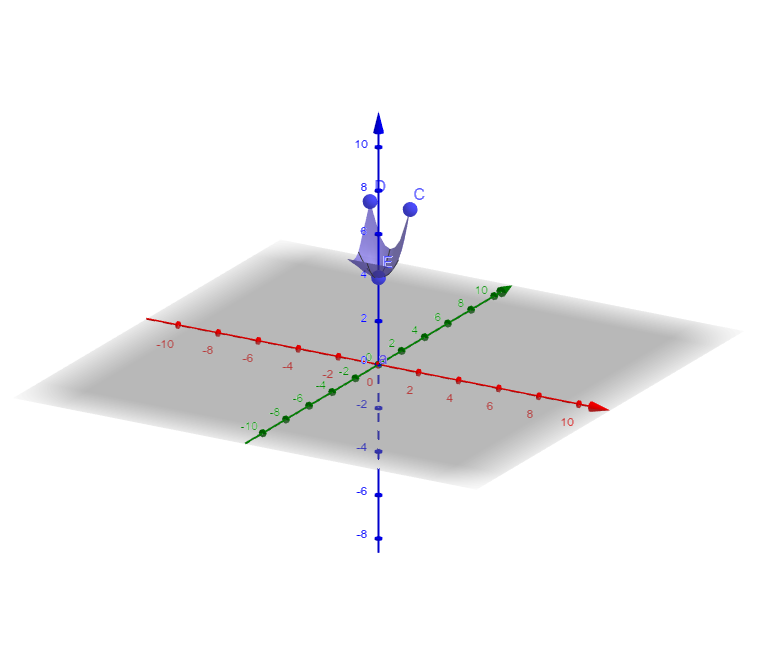
\includegraphics[scale=0.4]{ej05/resources/5b.png}$

        \item $f(x,y) = x^4+y^4-4xy+2 \wedge D=\{(x,y)\in \mathbb{R}^2: 0\leq x \leq 3 \wedge 0 \leq y \leq 5\}$

            \subsection*{Interior de $D$}

            \begin{itemize}
                \item $f_x(x,y) = 4x^3 - 4y$
                \item $f_y(x,y) = 4y^3 - 4x$
            \end{itemize}

            $\grad f(x,y) = (0,0) \Leftrightarrow$

            $\left \{\begin{array}{ll}
                4x^3 - 4y = 0 \Rightarrow 4y^9 - 4y = 4y(y^8 - 1) = 0 \Leftrightarrow y \in \{0,1,-1\}\\
                4y^3 - 4x = 0 \Rightarrow x = y^3 
            \end{array} \right. \Rightarrow$

            Ptos criticos $(0,0), (1,1), \stackrel{\notin D}{(1,-1)}$

            \subsection*{Borde de $D$}

            \subsubsection{S1}

            $f(0,y) = y^4 +2 = g(y) \wedge 0 \leq y \leq 5$

            $g^{\prime}(y) = 4y^3, (0,0)$

            \subsubsection{S2}

            $f(x,0) = x^4 +2 \Rightarrow (0,0)$

            \subsubsection{S3}

            $f(3,y) = 3^4 + y^4 - 12y + 2 = h(y)$

            $h^{\prime}(y) = 4y^3 - 12 = 0 \Leftrightarrow y = \sqrt[3]{3}$

            $\Rightarrow (3,\sqrt[3]{3})$

            \subsubsection{S3}

            $f(x,5) = x^4 + 5^4 - 20x +2 = i(x) $

            $i^{\prime}(x) = 4x^3 - 20 = 0 \Leftrightarrow x = \sqrt[3]{5}$

            $\Rightarrow (\sqrt[3]{5},5)$

            \subsection*{Ptos criticos}

            \begin{itemize}
                \item $(0,0) \Rightarrow f(0,0) = 2$
                \item $(1,1) \Rightarrow f(1,1) = 0$
                \item $(3,\sqrt[3]{3}) \Rightarrow f(3,\sqrt[3]{3}) = 70.02$
                \item $(\sqrt[3]{5},5) \Rightarrow f(\sqrt[3]{5},5) = 601.35$
                \item $(0,5) \Rightarrow f(0,5) = 627$
                \item $(3,5) \Rightarrow f(3,5) = 648$
                \item $(3,0) \Rightarrow f(3,0) = 83$
            \end{itemize}

            f alcanza su maximo en $(3,5)$ y su minimo en $(1,1)$

            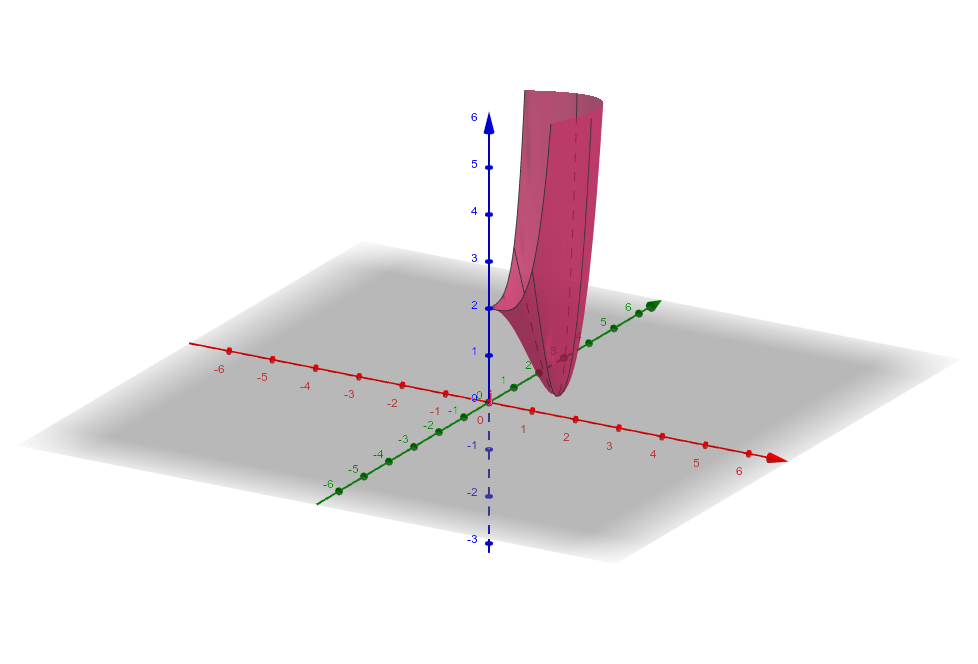
\includegraphics[scale=0.4]{ej05/resources/5c.png}

        \item $f(x,y) = xy^2 \wedge D=\{(x,y) \in \mathbb{R}^2: x \geq 0 \wedge y \geq 0 \wedge x^2+y^2 \leq 3 \}$
        
            \subsection*{Interior de $D$}

            \begin{itemize}
                \item $f_x(x,y) = y^2$
                \item $f_y(x,y) = 2xy$
            \end{itemize}

            $\grad f(x,y) = (0,0) \Leftrightarrow$
            
            $\left\{ \begin{array}{ll}
                y^2 = 0 \\
                2xy = 0
            \end{array}\right.$

            \subsection*{Borde de $D$}

            \subsubsection*{$x=0$}

                $f(0,y) = 0$

            \subsubsection*{$y=0$}

                $f(x,0) = 0$

            \subsubsection*{$x=\sqrt{3}\cos(t),y=\sqrt{3}\sin(t)$}

                $f(\sqrt{3}\cos(t),\sqrt{3}\sin(t)) = \sqrt{3}\cos(t)3\sin^2(t) = h(t)$

                $h^{\prime}(t) =  3\sqrt{3}(-\sin(t)\sin^2(t) + 2\sin(t)\cos^2(t)) \Rightarrow $

                $ -\sin(t)\sin^2(t) + 2\sin(t)\cos^2(t) = 0 \Leftrightarrow $

                $ t \neq 0 \Rightarrow 2\cos^2(t) = \sin^2(t) \Leftrightarrow $

                $ 2 = \frac{\sin^(t)}{\cos^(t)} \Leftrightarrow $

                $ 2 = (\frac{\sin(t)}{\cos(t)})^2 \Leftrightarrow $

                $ 2 = \tan^2(t) \Leftrightarrow $

                $ \sqrt{2} = \tan(t) \Leftrightarrow t = \arctan(\sqrt{2})$

                $\sqrt{0.88}$

                $ 0.955316618 $

            \subsection*{Pto criticos}

                \begin{itemize}
                    \item $P_1 = (0,0) \Rightarrow f(P_1) = 0 $ min
                    \item $P_2 = (\sqrt{3},0)\Rightarrow f(P_2) =0 $ min
                    \item $P_3 = (0,\sqrt{3})\Rightarrow f(P_3) =0 $ min
                    \item $P_4 = (\sqrt{3}\cos(\arctan(\sqrt{2})), \sqrt{3}\sin(\arctan(\sqrt{2})))\Rightarrow f(P_5) = 2$ max
                \end{itemize}

    \end{enumerate}

\end{document}
